\chapter{Introduction}
\label{cha:introduction}

Facial recognition systems are the applications capable of verifying or identifying a person based on the digital image. They have a wide range of usage such as identity authentication or security and access control.  Interest in this topic have increased significantly over the past decade, because it has potential to be the less invasive and user-friendly approach in human identification. Facial recognition applications become less expensive, making their use more widespread. Benefits of automatic facial recognition systems can be seen not only in security systems, but also in a commercial identification systems and marketing tools. We can unlock our phones using the facial recognition system, social media can tag people automatically on the uploaded pictures, even some dating sites match people with the same facial features using the theory that people are most attracted to those that look like them.

Although people seem to recognize faces relatively easy, automatic recognition is a much more daunting task. A capable face recognition system should be able to deal with variations of face images in viewpoint, illumination, and facial expression. This makes face recognition a great challenge. 

To visualize how hard this problem can be, some pictures of the same individual are presented on figure (??). Even though they all belong to the same person, they are hardly recognized as such, even by a human.

\begin{figure}[H]
\centering
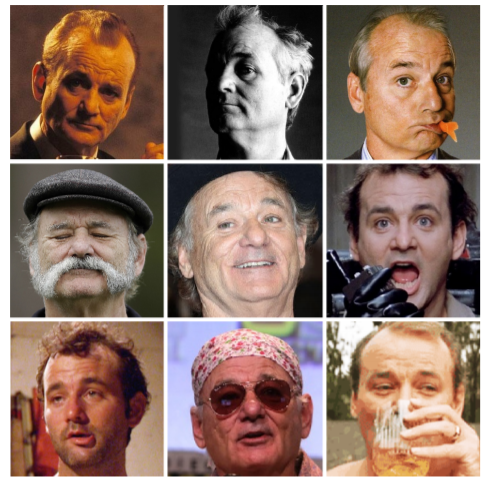
\includegraphics[scale=0.5]{img/the_same_person.png}
\caption{Very different pictures of a single individual}
\end{figure}


Facial recognition is an active area of research, spanning several disciplines such as image processing, pattern recognition, computer vision and neural networks. Engineering started to show interest in face recognition in the mid-1960’s. One of the pioneers in this topic was Woodrow W. Bledsoe. He developed a semi-automatic system that could classify photos of faces by hand using so-called a "RAND tablet" - a device that people could use to input horizontal and vertical coordinates on a grid using a stylus that emitted electromagnetic pulses. The system was used to record the coordinate locations of various facial features such as the eyes, nose, hairline or mouth. Gathered information were used by computers in further facial recognition. 


In 1988, Sirovich and Kirby applied the linear algebra to the problem of facial recognition, introducing the Eigenface approach. They showed that feature analysis on a collection of facial images could form a set of basic features. They were also able to show that less than one hundred values were required in order to accurately code a normalized face image. Few years later Turk and Pentland expanded the approach by discovering how to detect faces within images. This led to the first automatic face recognition. It was a real milestone in proving the feasibility of automatic facial recognition.

In the meantime another branch of study was being developed - the artificial neural networks. This, inspired by the human brain structure system turned out to be a breakthrough solution to many engineering problems. 

Nowadays, deep neural network approach is one of the most actively investigated method regarding the facial recognition problem. Deep Learning is at the cutting edge of what machines can do. It seems to provide the best results among all other facial recognition algorithms. 


%---------------------------------------------------------------------------


















